\section{Introduction and Goals}

According to the \acrfull{fao} in 2019 931 millions tonnes of food were wasted \cite{refart:FAOFW}. This has
environmental, but special social consequences. In a world were approximately 9.9\% of the \cite{refart:AAHWH}
population suffers from hunger that waste percentage sounds paradoxal.

According to \acrfull{un} 5\% of the globally food loss and waste comes from restaurants \cite{refart:UNSP}. 
The solution for this problem muss be locally applied so its effects can be seen in a global structure. To do so we
propose to develop a mobile application that connects restaurants, bakeries and or pastries to clients. 
The former would offer their remaining products, which are still consumable, prior to the closing time, to a small price 
and the latter would browser in the app to find which shops are offering products. 

 
\subsection*{Use cases}

The following use cases were defined according to the main purpose of the application:

% Object: put figure beside the table

\begin{table}[htb]
    \begin{tabularx}{\textwidth}{lX}
    \toprule
    Use Case & Description  \\
    \midrule
    UC-1: Register as client & The user register an e-mail address.\\
    UC-2: Login & The user logins in to the system. \\
    UC-3: Place order & The user chooses a provider. \\
    UC-4: Register payment & The user register a payment method. \\
    UC-5: Register as provider & The provider register their facility and products. \\
    UC-6: Update availability & The provider upload their availability to provide a product. \\
    \bottomrule
    \end{tabularx}
\end{table}

\begin{figure}[htb]
    \centering
    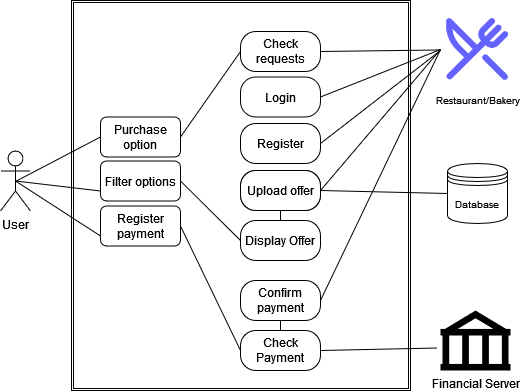
\includegraphics[width=0.50\textwidth]{/home/bruno/git/Soft.Arch/assets/preliminary_use_case.png}
    \caption{Preliminary functions}
    \label{fig:predes}
\end{figure}


\subsection*{Quality Attributes}

\begin{table}[H]
\begin{tabularx}{\textwidth}{lcXc}
    \toprule
    ID & Quality Attribute & Scenario & Associated Use Case  \\
    \midrule
    QA-1 & 123 & A client register their e-mail address and he can immediate browse in the app. & UC-1 \\
    QA-2 & 123 & A client login in the app and he can immediate browse in the app. & UC-2 \\
    QA-3 & 123 & A client choose a provider and place his order. After the confirmation
    of payment, a push-message is displayed in the app confirming the purchase. & UC-3 \\
    QA-4 & 123 & A client register his credit card or select another payment method and the
    confirmation as soon as he confirmed with his provider. & UC-4 \\
    QA-5 & 123 & A provider is able to register his company, specify the kind of products he offers and upload
    a logo or picture of his shop. & UC-05 \\
    QA-6 & 123 & A provider is able to update in the app if he is offering for that day any product. &  UC-6 \\
    \bottomrule
\end{tabularx}
\end{table}




\begin{itemize}
    \item \textit{Usuability}: Offering and selecting options should be intui
    \item \textit{blablabla}
    \item \textit{blablabla}
\end{itemize}


Check Add 3.0
Check FAO for reasoning
Define Drivers:

\begin{itemize}
    \item Design Purpose: prototype, check acceptance
    \item Quality
    \item Primary Functionality: realy first to get the system to start, food ordering, registering, offering
    \item Constraints: laws, deadlines, standards
    \item Concerns: can be left blank
\end{itemize}

pick 3 qualities

Quality: A ==> Create Scenarios ==> Prioritize High, Medium, Low for (Arch, Customer)
Quality: usability ==> Create Scenarios ==> Prioritize (for Arch, for Customer) 
Quality: availability ==> Create Scenarios 
Quality: modifiability ==> Create Scenarios
Quality: security ==> Create Scenarios

% https://www.ecs.csun.edu/~rlingard/COMP684/Example2SoftArch.htm
% https://upcommons.upc.edu/bitstream/handle/2099.1/18373/90629.pdf

% \subsection*{Qualities}
% Usability
% \begin{itemize}
%     \item Design Purpose: prototype, check acceptance

% \end{itemize}

% UC-1: Register - Users register themselfeves
% UC-2: Login - User should be able to login themselves
% UC-3: Upload offer - Restaurants upload in the app that they are offering products
% UC-4: Purchase - Clients pick a Restaurant and purchase the product
% UC-5: 



% Usuability
% QA1 - Usuability - Users should be able to register themselfeves easily
% QA2 - Usuability - The interfaces are intuitive to use (learning)
% QA3 - Performance - Users recieve answer quickly after taking decisions

% Registration Process for Clients QA1
% Registration Process for Restaurants/Backery QA2
% Login Clients QA3
% Login Restaurant/Backery QA4
% Upload offers QA6
% Purchase QA6
% Receive Confirmation QA7

% Performance
% After upload offer, how long until displyed QA8




% Usuability
% Registration for Client: using existing account or Name/email
% Registration for Restaurant/bakery: Upload name, picture, location and type of products

% Purchase client: choose available RA-options
% Payment: register card, use existing accounts (paypal/google pay)

% Upload offer RA: registered RAs activate that they are offering
% Receive order: after payment confirmed, RA recieves order


% Availability

% Source: Client
% Stimulus: Register
% System: Federation (using existing logins from other platforms, google/facebook etc)
% Response: Accounted create + display options
% Response Measure: Register should be performed only once


% Source: Client
% Stimulus: open application
% System: Mobile-Application
% Response: Display available options
% Response Measure: options are updated every xx Minutes


% Source: Client
% Stimulus: choose restaurant/bakery
% System: Mobile-Application
% Response: Push-message with confirmation
% Response Measure: The purchase is automatically displayed


% Source: Restaurant
% Stimulus: Registers
% System: Mobile-Application
% Response: Restaurant Name
% Response Measure: After sending info, available on the application in up to 5 minutes

% Source: Restaurant
% Stimulus: Upload offer
% System: Mobile-Application
% Response: On the app the offers available in the restaurant/bakery are displayed
% Response Measure: After sending info, available on the application in up to 5 minutes


% Source: Client
% Stimulus: Purchase
% System: Mobile-Application
% Response: Restaurant/bakery receive order from client
% Response Measure: Time between payment and confirmation to restaurant/bakery


% Source: Restaurant
% Stimulus: remove offer
% System: Mobile-Application
% Response: Customer and Restaurant no longer see the Item in their List
% Response Measure: Updates should be delivered within 2 minutes after sending


% Modifiability
